\begin{figure}[!ht]
  \centering
  % https://docs.google.com/presentation/d/109vfeK_lHSsE0q7Iz7tzl9sDxnP8jyOF2gJ-v85pgL8/edit?usp=sharing
  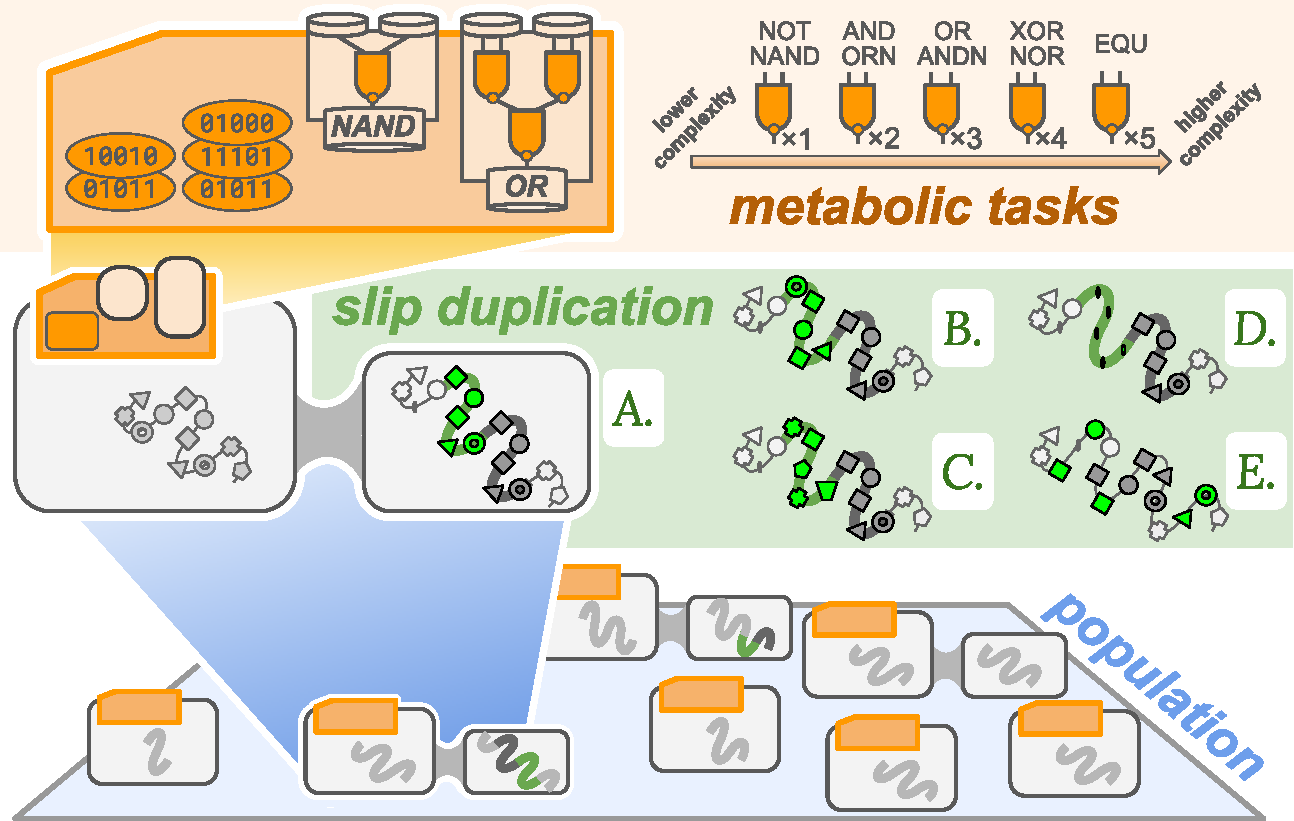
\includegraphics[height=0.6\linewidth, angle=90]{imgs/GeneDupeOps.pdf}
    \caption{
    \textbf{Surveyed slip mutation operators.}
    A) Slip-duplicate: an exact duplication is inserted adjacent to the target segment.
    B) Slip-scramble: shuffled duplication is inserted directly after the target segment.
    C) Slip-random: random instructions are inserted directly after the target segment.
    D) Slip-NOP: neutral nop-X instructions are inserted directly after the target segment.
    E) Slip-scatter: randomly-drawn instructions are inserted at random throughout the genome.
    }
    \label{fig:slip_mut_variants}
\end{figure}
